\chapter{Project Management}\label{project-management}

\section{Software Development Process}

An agile approach based on RUP has been used as the process model of this project. At the kickoff meeting the schedule with the milestones were defined and the first tasks were assigned to the alpha milestone. In frequent meetings the progress of these tasks were tracked and new tasks were created.\\
Constant evolution has been favored over long term planning and this approach has proven itself for this type of work, where unexpected problems are the rule not the exception.

\subsection{Github}\label{github}
Github was used for planning and tracking of the tasks and milestones. It has a big advantage over other project management tools, as the revision control and the issue tracking is at the same place. Non project members can understand the thoughts behind certain decisions and communicate their ideas directly to team members.\\
An organization named osm2vectortiles was created with the following two repositories:

\begin{itemize}
\item
  \textbf{osm2vectortiles} contains the project\footnote{\url{https://github.com/osm2vectortiles/osm2vectortiles}}
\item
  \textbf{osm2vectortiles-thesis} contains the thesis\footnote{\url{https://github.com/osm2vectortiles/osm2vectortiles-thesis}}
\end{itemize}

\section{Schedule}

Compared to other software projects a much longer elaboration phase has been chosen. In the elaboration the most difficult problems have been solved with a prototype which was then refined in the construction phases. Due to the many risks regarding rendering time and unknown technology problems the longer elaboration phase really helped to eradicate risks early on.

\begin{figure}[H]
  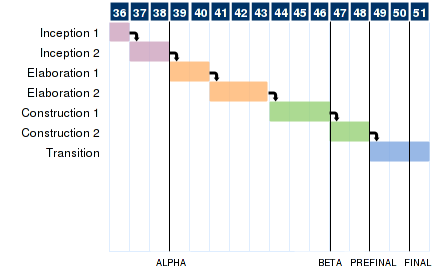
\includegraphics[scale=0.9]{images/phasen.png}
  \caption{Phases during project}
\end{figure}

\section{Milestones}

Each milestones marks a special release version of the vector tiles.

\begin{table}[H]
    \begin{tabular}{p{2.5cm} p{10cm}}
    ALPHA &  Proof of concept tileserver.\\ \hline
    BETA &  Switzerland with upper zoom levels.\\ \hline
    PREFINAL &  Switzerland with lower zoom levels.\\ \hline
    FINAL &  Improved and polished final release. \\ \hline
    \end{tabular}
    \caption[Milestones]{Project milestones}
\end{table}


\section{Project Stages}\label{project_stages}

\begin{table}[H]
    \begin{tabular}{p{2.5cm} p{10cm}}
	Inception 1 & Kickoff meeting and
  definition of project proposal. \\ \hline

	Inception 2 & Getting familiar with the entire Mapbox stack and create a very basic prototype of every deliverable on a small scale. \\ \hline

	Elaboration 1 & Evaluation of different parts of the
  stack like import tools and vector tile server.  \\ \hline
  Elaboration 2  & Prototype of import and export components
\\ \hline

  Construction 1 & Custom data style up from zoom level 8 to 14  \\ \hline

  Construction 2 & Custom data style up from zoom level 0 to 8 \\ \hline
  Transition & Rendering and preparing the vector tiles and time for documentation and project website.\\ \hline
    \end{tabular}
    \caption{Project stages}
\end{table}

\section{Roles and Responsibilities}\label{roles-and-responsibilities}

\begin{table}[H]
    \begin{tabular}{p{3cm} p{9.5cm}}
Prof Stefan Keller & Thesis advisor responsible for supervising work and
assess the thesis.\\ \hline
Dr Petr Pridal &
Technical partner responsible for providing infrastructure and guidance in technical and map related questions.\\ \hline
Manuel Roth &
Contributor responsible for data style and JavaScript tooling.\\ \hline
Lukas Martinelli &
Contributor responsible for rendering infrastructure and Python scripts.\\ \hline
    \end{tabular}
    \caption{Thesis contributors and their roles}
\end{table}

\section{Risks}\label{risks}
In general this project was hazardous, as not a lot of cartographic knowledge was present at the beginning. The risk was reduced by contacting our advisors early, when ever problems appeared. The knowledge gap was filled very fast, due to the availability of superb information sources online. The figure below shows only project specific risks, which have been assessed and dealt with accordingly.

\begin{table}[H]
    \begin{tabular}{p{3.5cm} p{7.5cm} p{1.8cm}}
    \hline
    Risk & Measurement & Probability (1-6)\\
    \hline
    Low cartographic knowledge & Start earlier for additional training time & 6\\
    Rendering takes too long & Increase infrastructure & 5\\
    Infrastructure not sufficient & Switch to non school infrastructure and rely on external sponsors & 3\\
    No community acceptance & Meet early with OSM community & 3\\
    Quality not sufficient & Invest sufficient time in perfecting the quality & 3\\
    High technical complexity & Prototype early & 6\\
    Insufficient tracking of project progress & More frequent meetings & 2\\
    \end{tabular}
    \caption{Risks and measurements}
\end{table}

\paragraph{High technical complexity} The project involved a lot of different technologies, as we built up a whole workflow to produce vector tiles. As a measurement the elaboration phase was used to create a first working prototype, which should prove the implementation concept.

\paragraph{Insufficient tracking of project progress} The project progress was tracked on Github, so the progress was at any time publicly visible. Regular meetings with our advisors helped staying focused on the project goals.

\paragraph{Infrastructure not sufficient} The rendering process of vector tiles is a very ressource intense task. The school infrastructure was not enough to fulfill the project goals in time. Therefore an alternative platform with more processing power was used to complete the rendering task in time.\\

As this project brought up new challenges every day, not all of the risks could be eliminated during the elaboration phase. Measurements had to be found, when ever new risks appeared.

%---------------------------------------------------------------
\newpage
\chapter{Quality Measures}\label{quality-measures}

\section{Testing}\label{testing}

The osm2vectortiles ecosystem is quite diverse with a big collection of small tools that all work together.

\section{Debug Viewer}

During development the tiles were continuously examined with the Mapbox Studio Classic debug viewer.
This tool makes it possible to verify the different attributes of features and ensure the queries deliver the right results.

\begin{figure}[H]
  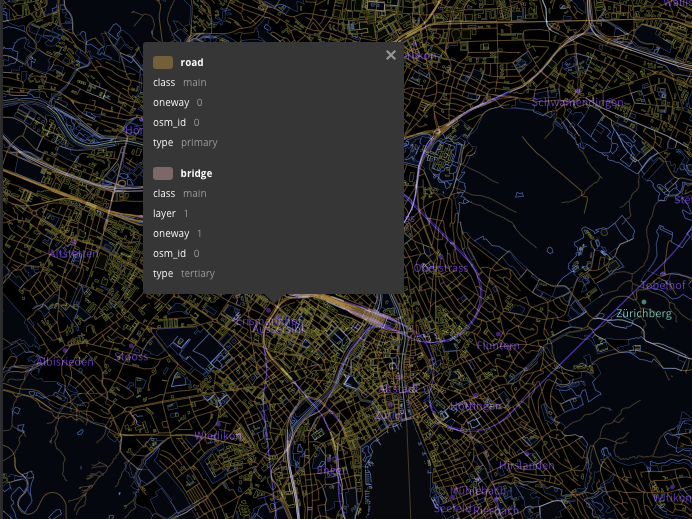
\includegraphics[width=1\textwidth]{images/mapbox_studio_debug_viewer.png}
  \caption{Mapbox Studio Classic Debug Viewer}
\end{figure}

The Open Source partner Klokan Technologies \footnote{\url{http://www.klokantech.com/}} also provided a OpenLayers 3\footnote{\url{http://openlayers.org/}} based debug viewer,
which supports the same features but allows looking at arbitrary TileJSON urls.

\begin{figure}[H]
  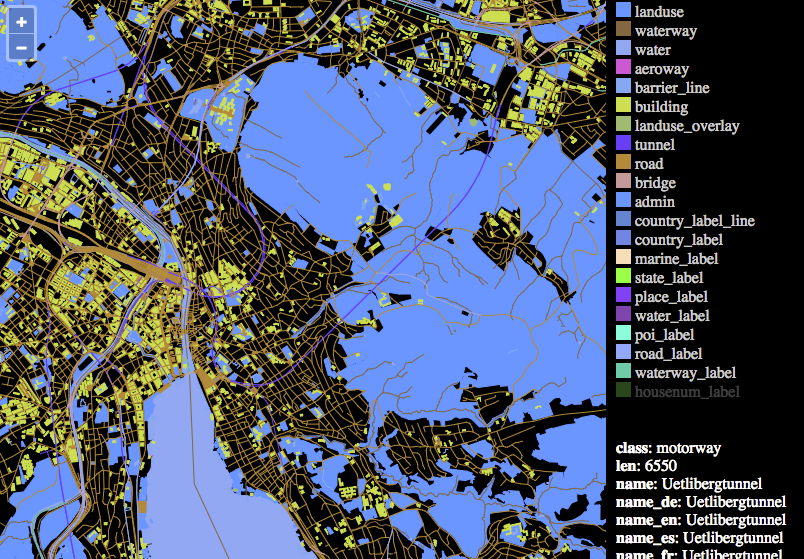
\includegraphics[width=1\textwidth]{images/klokantech_debug_viewer.png}
  \caption{Klokantech Debug Viewer}
\end{figure}
The tile inspector is another tool by Klokan Technologies which supports inspecting vector tile PBFs for their size and features and visually explore the structural features of the \nameref{vector_tile_compare}.

\begin{figure}[H]
  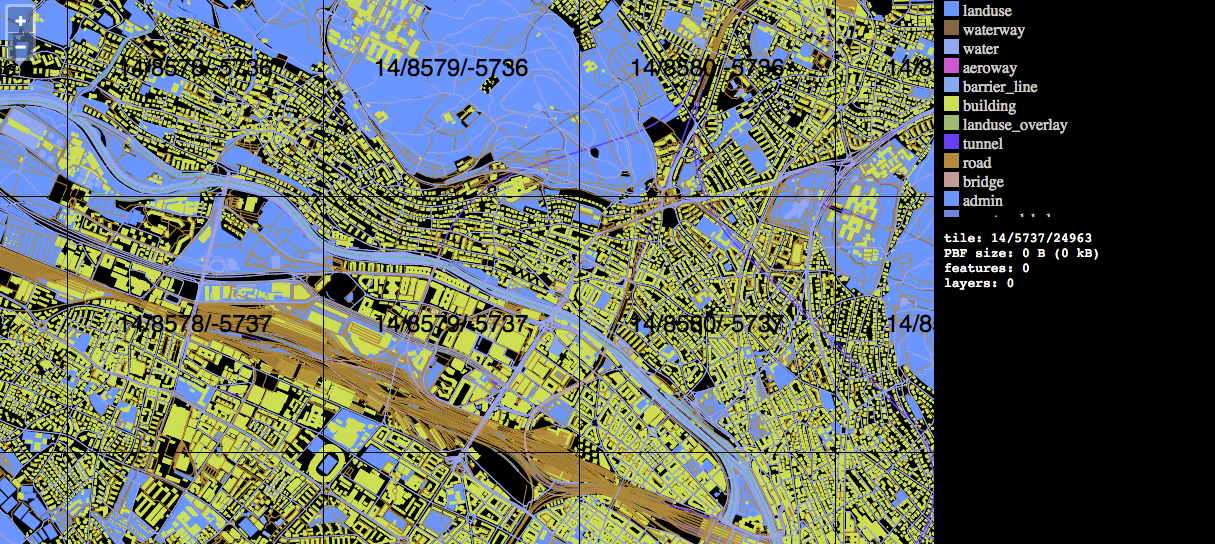
\includegraphics[width=1\textwidth]{images/klokantech_tile_inspector.png}
  \caption{Klokantech Tile Inspector}
\end{figure}



\section{Visual Test}

The \nameref{visual_compare} tool allowed to preview the map visually and compare the rendered raster tiles directly with Mapbox Streets.

\section{Structural Test}

With the \nameref{vector_tile_compare} tool the differences between Mapbox Streets and the Open Streets vector tiles were regularly compared by hand. This tool was used as guidance for reverse engineering and ensuring the same feature classes appear at the same zoom levels.

\section{Integration Test}

In Travis CI\footnote{\url{travis-ci.org}}  the entire workflow was completed for a small data sample on each commit.
Because the entire workflow is configured with Docker Compose \footnote{\url{https://docs.docker.com/compose/}} the CI server had to execute all import steps in serial order. This is a straightforward way to check if all components work together correctly
and although it is a simple setup it has helped tremendously during project development, catching bugs
like missing tables or SQL typos.

\begin{yamlcode}
script:
  - docker-compose up -d postgis
  - docker-compose up -d pgbouncer
  - docker-compose run import-osm
  - docker-compose run import-natural-earth
  - docker-compose run import-water
  - docker-compose run import-labels
  - docker-compose run import-sql
  - docker-compose run update-scaleranks
  - docker-compose run export-local
  - docker-compose up -d serve
  - curl "http://localhost:8080/index.json"
\end{yamlcode}



\section{Guidelines}\label{guidelines}
To have homogeneous software we settled on common guidelines in the beginning of the project.

\subsection{Releases}
We use semantic versioning \footnote{\url{http://semver.org/}}. At the
end of each milestone a new release will be created.

\subsection{Git}\label{git}
\paragraph{Commit Messages}
We use the seven rules of great git commit
messages\footnote{\url{http://chris.beams.io/posts/git-commit/}}.

\paragraph{Rewriting}
Git history should be kept clean and therefore local branches should be
squashed meaningfully.

\paragraph{Pulling}
To avoid unnecessary merge messages one should always use the
\texttt{-\/-rebase} parameter.

\subsection{Workflow}\label{workflow}
We use the Feature Branch Workflow\footnote{\url{https://www.atlassian.com/git/tutorials/comparing-workflows/feature-branch-workflow/}}.

Every project member has a local repository with a copy of the remote
repository. For each feature ticket in GitHub a separate branch
will be created. Once a ticket has been completed a pull request will be
created and needs to be merged into the \texttt{master} branch by an other 

\subsection{Coding Standards}

\paragraph{Bash} We use Bash for our Docker image entrypoints and follow
the rules of Defensive Bash Programming \footnote{\url{http://www.kfirlavi.com/blog/2012/11/14/defensive-bash-programming/}}.

\paragraph{Python} For Python code we want to stay PEP-8\footnote{\url{https://www.python.org/dev/peps/pep-0008/}} compliant and write idiomatic Python code according to PEP-20\footnote{\url{https://www.python.org/dev/peps/pep-0020/}}.

\paragraph{JavaScript} The JavaScript code is checked using ESLint\footnote{\url{http://eslint.org/}}

\paragraph{SQL} Our PostgreSQL code is using upper case for the key words. Apart from that we try to have nice formatted SQL code and use functions
if necessary to keep the queries DRY\footnote{\url{https://en.wikipedia.org/w/index.php?title=Don%27t_repeat_yourself&oldid=691047461}}.

\paragraph{Dockerfile} Dockerfiles follow the best practices\footnote{\url{https://docs.docker.com/engine/articles/dockerfile\_best-practices/}} defined by Docker.

%---------------------------------------------------------------